\section{Durchführung}
\label{sec:Durchführung}
Die Apparatur wird wie in \autoref{fig:Versuchaufbau} dargestellt aufgebaut. In den XY-Schreiber wird
Millimeterpapier eingelegt und der XY-Schreiber auf die entsprechende Messreihe eingestellt.
\begin{figure}
    \centering
    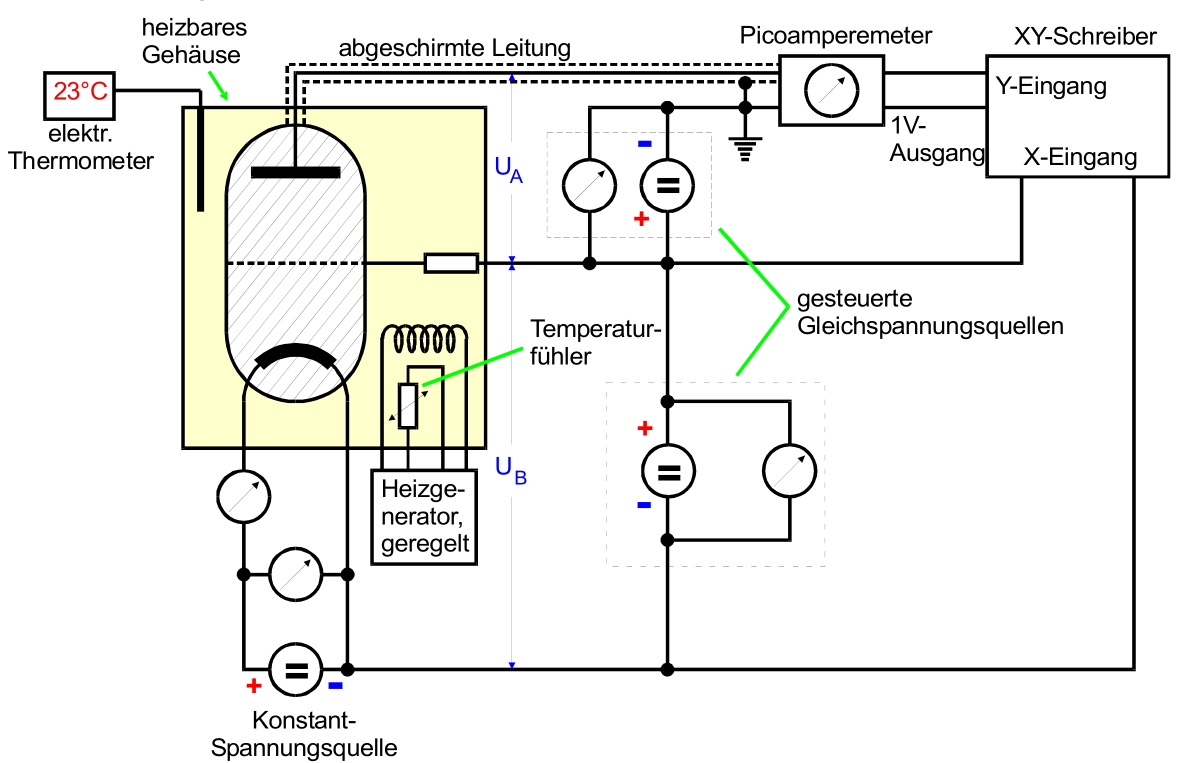
\includegraphics[width=0.7\textwidth]{Bilder/Versuchsaufbau.png}
    \caption{Darstellung des Versuchaufbaus \cite{sample}.}
    \label{fig:Versuchaufbau}
\end{figure}
Bei der ersten Messreihe wird die Beschleunigungsspannung konstant bei $11\,\unit{\volt}$ gelassen und der
Auffängerstrom in Abhängigkeit der Bremsspannung gemessen. Es wird jeweils eine Messung bei
$27\,\unit{\celsius}$ und bei $160\,\unit{\celsius}$ gemacht. Bei der zweiten
Messreihe werden nun zwei Franck-Hertz Kurven für zwei Temperaturen von $175\,\unit{\celsius}$ und
$185\,\unit{\celsius}$ aufgenommen. Dazu wird die Bremsspannung auf $1\,\unit{\volt}$ gesetzt und der
Auffängerstrom in Abhängigkeit der Beschleunigungsspannung gemessen.